\section{Arquitectura completa del CANae}
CANae nace en el principio de la ingeniería en sistemas basada en modelo
utilizando el lenguaje de modelado SysML para su diseño y desarrollo.
Debido a la complejidad de los sistemas espaciales, a la
necesidad de lograr un entendimiento completo por parte de los desarrolladores,
y para lograr un correcta interpretación del protocolo se decidió basarse en
este principio. En esta sección se pretende mostrar solo con motivo informativo
la arquitectura estáttica completa del protocolo, para demostrar la complejidad
del mismo, pero a la vez lo sencillo que resulta su interpretación, con
conocimientos básicos de SysML.

En esta se puede observar como interactúan las diferentes entidades, objetos y
eventos que se desarrollaron a lo largo de este documento.

En la Figura \ref{fig:Arq_CAN_App_Layer} se observa la arquitectura de la capa
de aplicación de CANae denominada: \textbf{CAN Application Layer CANae}. La cual
como se mencionó con anterioridad se encuentra basada en la capa de aplicación
de diferentes protocolos que existen para las redes CAN.

\begin{sidewaysfigure}[h!]
  %\begin{figure}[h!]
    \centering
    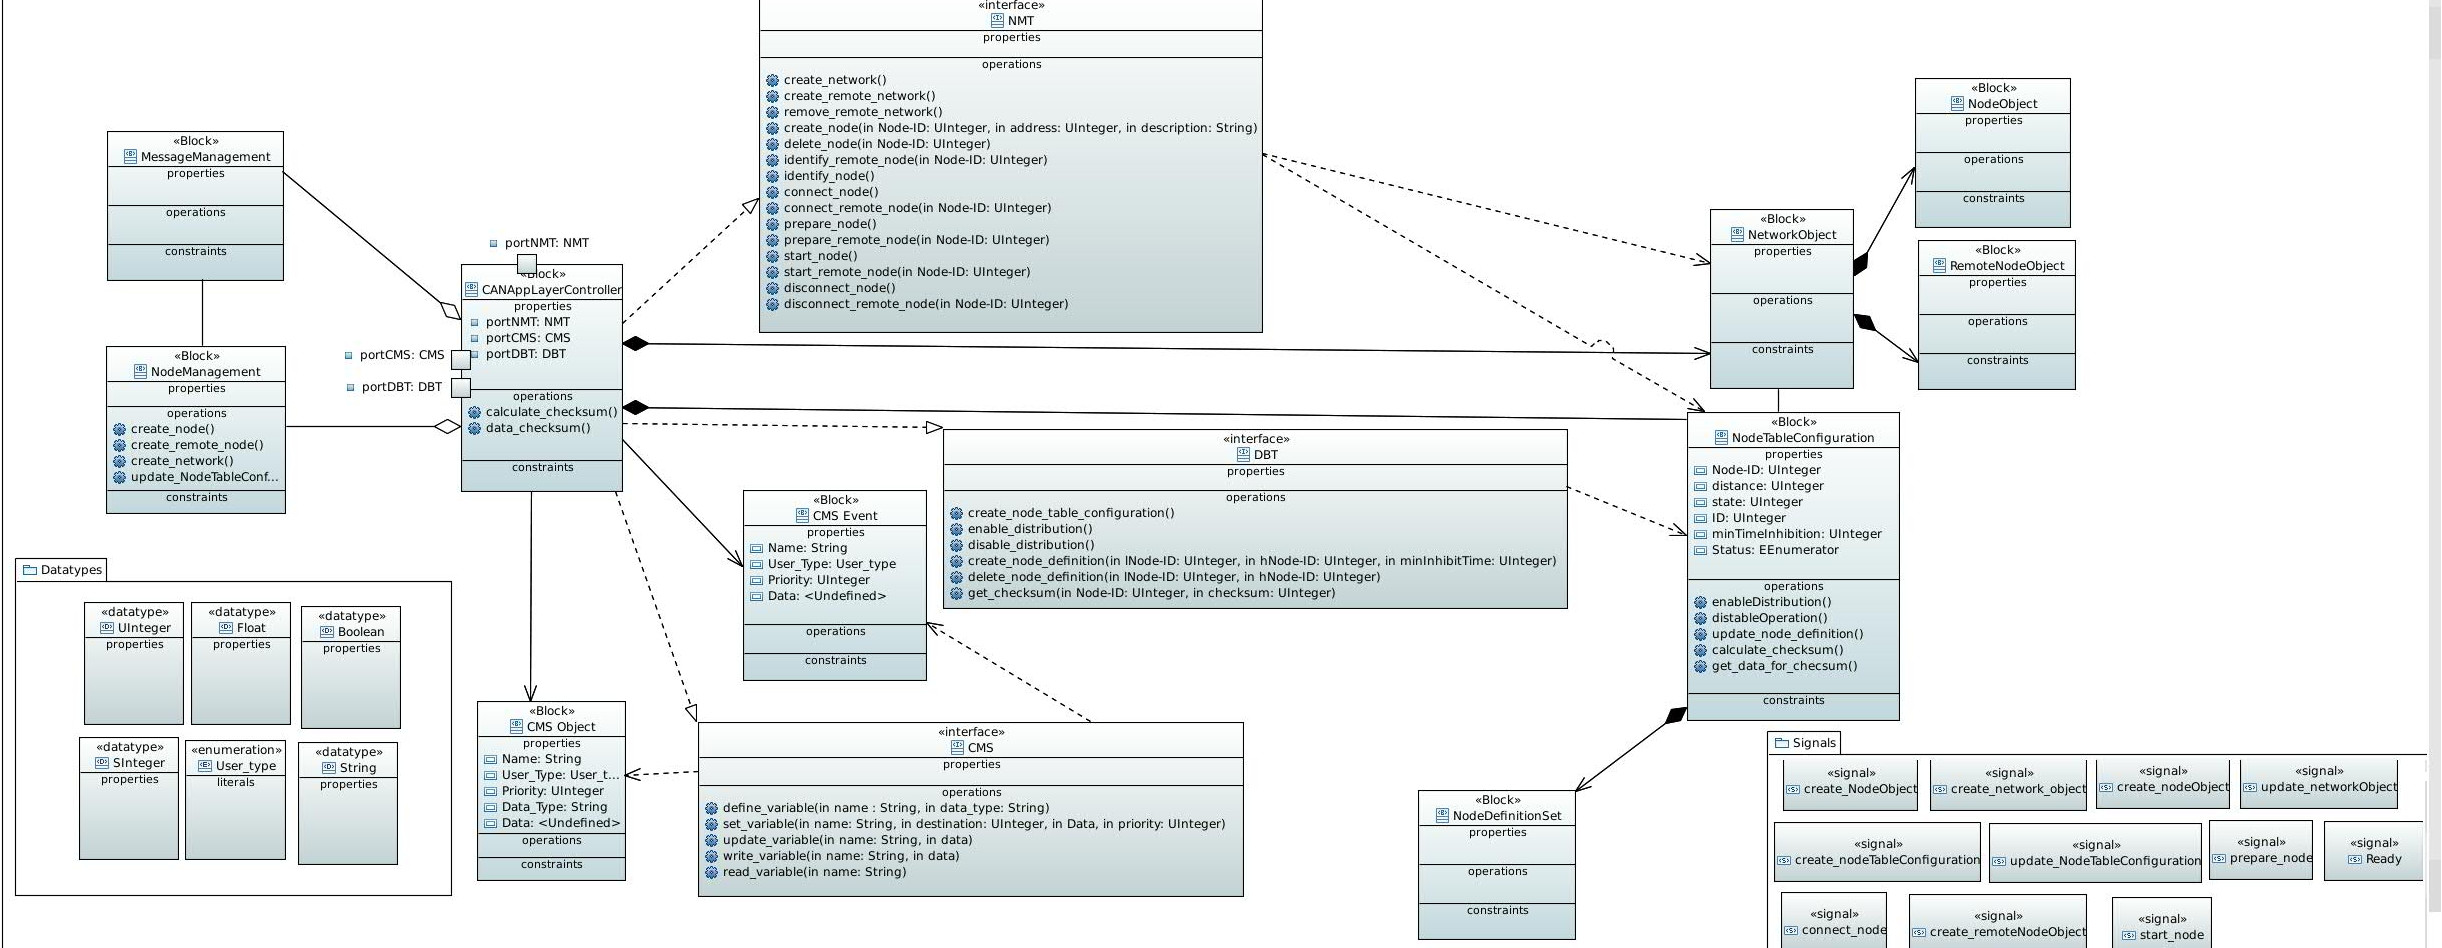
\includegraphics[scale=0.25]{images/Secciones/AppendixA/Complete_CANAppLayerCANae2.JPG}
    \caption{Arquitectura completa del CANae}
    \label{fig:Arq_CAN_App_Layer}
  %\end{figure}
\end{sidewaysfigure}
